\documentclass[UTF8]{ctexart}
\usepackage{amsmath,amssymb,graphicx}

%%%%%%%%%% Start TeXmacs macros
\newcommand{\tmop}[1]{\ensuremath{\operatorname{#1}}}
\newcommand{\tmscriptoutput}[4]{#4}
%%%%%%%%%% End TeXmacs macros

\begin{document}

\

\title{2019年全国高中数学联合竞赛一试试题(A卷)}

\maketitle

\subsection*{一、填空题:本大题共8小题,每小题8分,满分64分。}

\begin{enumerate}
  \item 已知正实数$a$满足$a^a = (9 a)^{8 a}$,则$\log_a (3
  a)$的值为{\underline{{\hspace{3em}}}}.
  
  \item 若实数集合$\{ 1, 2, 3, x
  \}$的最大元素与最小元素之差等于该集合的所有元素之和,则$x$的值为{\underline{{\hspace{3em}}}}.
  
  \item
  平面直角坐标系中,$\vec{e}$是单位向量,向量$\vec{a}$满足$\vec{a}
  \cdot \vec{e} = 2$,且$| \vec{a} | \leqslant 5 | \vec{a} + t \vec{e}
  |$对任意实数$t$成立,则$| \vec{a}
  |$的取值范围为{\underline{{\hspace{3em}}}}.
  
  \item 设$A, B$为椭圆$\Gamma$的两个焦点,$| \tmop{AB} | = 4$,$|
  \tmop{AF} | = 2 + \sqrt{3}$,$P$为$\Gamma$上一点,满足$| \tmop{PE} |
  \cdot | \tmop{PF} | = 2$,则$\Delta
  \tmop{PEF}$的面积为{\underline{{\hspace{3em}}}}.
  
  \item 在$1, 2, 3, \ldots, 10$中随机选出一个数$a$,在$- 1, - 2, -
  3, \ldots, - 10$中随机选出一个数$b$,则$a^2 +
  b$被3整除的概率为{\underline{{\hspace{3em}}}}.
  
  \item 对任意闭区间$I$,用$M_I$表示函数$y = \sin
  x$在$I$上的最大值.若正数$a$满足$M_{\{ 0, a \}} = 2 M_{\{ a, 2 a
  \}}$,则$a$的值为{\underline{{\hspace{3em}}}}.
  
  \item 如图,正方体$\tmop{ABCD} -
  \tmop{EFGH}$的一个截面经过顶点A,
  C及棱EF上一点K,且将正方形分成体积比为3:1的两部分,则$\frac{\tmop{EK}}{\tmop{KF}}$的值为{\underline{{\hspace{3em}}}}.
  
  \tmscriptoutput{asymptote}{Asymptote}{\% -width 270
  
  import three;
  
  \
  
  size (100);
  
  \
  
  triple
  
  D= (0,0,0),
  
  A= (1,0,0),
  
  B= (1,1,0),
  
  C= (0,1,0),
  
  H= (0,0,1),
  
  E= (1,0,1),
  
  F= (1,1,1),
  
  G= (0,1,1),
  
  K= (1, 2/3, 1);
  
  
  
  dot("\$A\$", A, NE);
  
  dot("\$B\$", B, NE);
  
  dot("\$C\$", C, NE);
  
  dot("\$D\$", D, NE);
  
  dot("\$E\$", E, NE);
  
  dot("\$F\$", F, NE);
  
  dot("\$G\$", G, NE);
  
  dot("\$H\$", H, NE);
  
  dot("\$K\$", K);
  
  \
  
  \
  
  draw (A--B--C);
  
  draw (D--A, dotted);
  
  draw (D--C, dotted);
  
  draw (D--H, dotted);
  
  draw (A--E);
  
  draw (B--F);
  
  draw (C--G);
  
  draw
  (E--F--G--H--cycle);}{\raisebox{0.0\height}{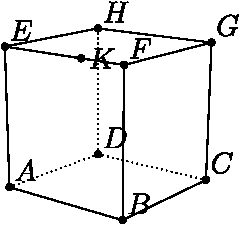
\includegraphics[width=5.667060212514758cm,height=5.3165092483274305cm]{2019年全国高中数学联合竞赛一试试题A卷-1.pdf}}}
  
  \item 将6个数$2, 0, 1, 9, 20,
  19$按任意次序排成一行,拼成一个8位数(首位不为0),则产生的不同的8位数的个数为{\underline{{\hspace{3em}}}}.
\end{enumerate}

\subsection*{二、解答题:本大题共3小题,满分56分。解答应写出文字说明、证明过程或演算步骤。}

\begin{enumerate}
  \item (本题满分16分)在$\Delta \tmop{ABC}$中,$\tmop{BC} =
  a$,$\tmop{CA} = b$,$\tmop{AB} =
  c$.若b是a与c的等比中项,且$\sin A$是$\sin (B - A)$与$\sin
  C$的等差中项,求$\cos B$的值.
  
  \item
  (本题满分20分)在平面直角坐标系$\tmop{xOy}$中,圆$\Omega$与抛物线$\Gamma
  : y^2 = 4
  x$恰有一个公共点,且圆$\Omega$与$x$轴相切于$\Gamma$的焦点$F$,求圆$\Omega$的半径.
  
  \item (本题满分20分)称一个复数数列$\{ z_n
  \}$为``有趣的'',若$| z_1 | = 1$,且对任意正整数n,均有$4
  z_{n + 1}^2 + 2 z_n z_{n + 1} + z_n^2 =
  0$,求最大的常数$C$,使得对一切有趣的数列$\{ z_n
  \}$及任意正整数$m$,均有$| z_1 + z_2 + \cdots + z_m | \geqslant C$.
\end{enumerate}

\end{document}
